\documentclass{article}%
\usepackage[T1]{fontenc}%
\usepackage[utf8]{inputenc}%
\usepackage{lmodern}%
\usepackage{textcomp}%
\usepackage{lastpage}%
\usepackage[head=40pt,margin=0.5in,bottom=0.6in]{geometry}%
\usepackage{graphicx}%
%
\title{\textbf{Detuvieron a concejal del municipio Libertador en Maiquetía}}%
\author{El Nacional Web}%
\date{05/10/2018}%
%
\begin{document}%
\normalsize%
\maketitle%
\textbf{URL: }%
http://www.el{-}nacional.com/noticias/politica/detuvieron{-}concejal{-}del{-}municipio{-}libertador{-}maiquetia\_254513\newline%
%
\textbf{Periodico: }%
EN, %
ID: %
254513, %
Seccion: %
Política\newline%
%
\textbf{Palabras Claves: }%
NO\_TIENE\newline%
%
\textbf{Derecho: }%
1.2, %
Otros Derechos: %
1.10, %
Sub Derechos: %
1.2.2, 1.10.1\newline%
%
\textbf{EP: }%
NO\newline%
\newline%
%
\textbf{\textit{Fernando Albán de Primero Justicia asistió esta mañana a las manifestaciones de los trabajadores de diferentes gremios}}%
\newline%
\newline%
%
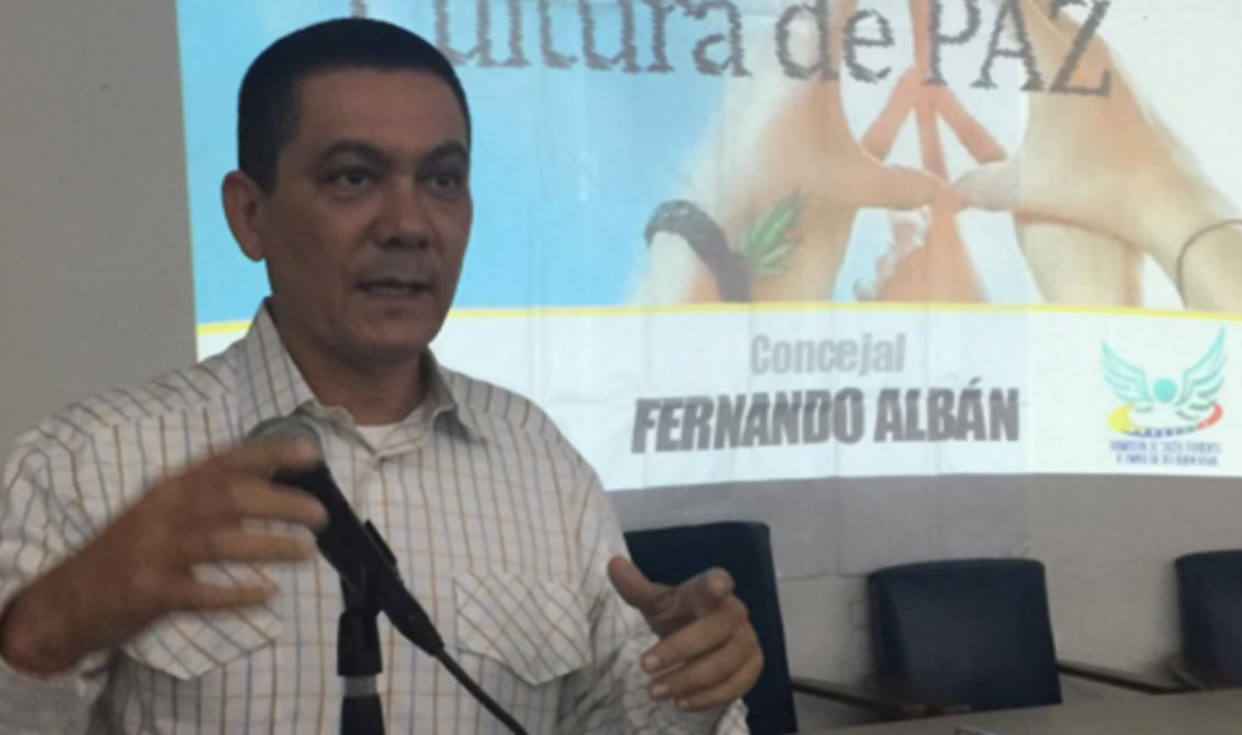
\includegraphics[width=300px]{152.jpg}%
\newline%
%
Este viernes en horas de la tarde funcionarios del Servicio Bolivariano de Inteligencia Nacional (Sebin) detuvieron al concejal del municipio Libertador, Fernando Albán, en el aeropuerto Internacional Simón Bolívar ubicado en Maiquetía, estado Vargas.%
\newline%
%
El concejal asistió esta mañana a las protestas de los trabajadores de diferentes gremios, que manifestaban por la violación de los contratos colectivos.%
\newline%
%
“Hace minutos Fernando Albán fue detenido por el Sebin en el aeropuerto de Maiquetía. Exigimos la inmediata liberación del concejal del partido Primero Justicia”, informó Tomás Guanipa, diputado a la Asamblea Nacional.%
\newline%
%
Primero Justicia (PJ) informó que responsabiliza a Nicolás Maduro por la integridad física de Albán.%
\newline%
%
\end{document}